\chapter{Profilo elettrico}

\section{Setup misure tensione e corrente}

\section{Misure ed analisi}
\paragraph{Tensione} Ogni set di misure viene processato eseguendo la trasformata di Fourier del segnale (usando le routine fftw3 delle librerie ROOT), tagliando le oscillazioni ad alta frequenza e ricostruendone una media. L'obiettivo è di migliorare la stima della posizione del minimo del picco andando ad escludere le oscillazioni a frequenza molto alta del ciruito.
A queste misure viene aggiunto l'errore dovuto al taglio delle alte frequenze, preso come una media del valore assoluto dell'oscillazione del segnale tagliato. Viene inoltre aggiunto l'errore caratteristico dello strumento di misura, ma è trascurabile rispetto le oscillazioni veloci.
Il valore del minimo viene trovato interpolando il set di misure attorno il minimo con una funzione di Landau, in modo da riprodurre l'asimmetria del picco. Da questo fit viene calcolato il massimo.
In figura \ref{fig:landau} un esempio del fit.

\begin{figure}
\centering
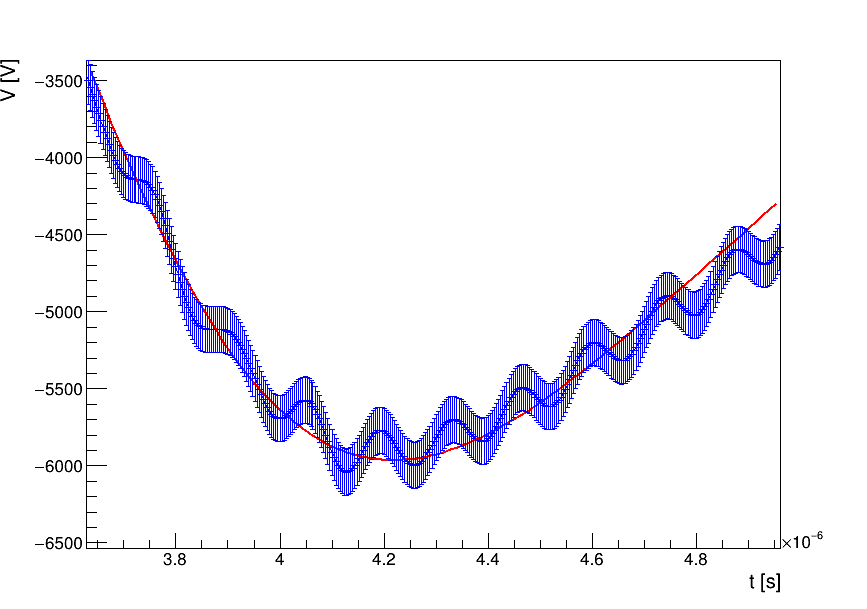
\includegraphics[width=.6\textwidth]{Immagini/esfiterr.png}
\caption{Esempio di fit del picco di tensione, $f = \SI{5}{\kilo\hertz}$ e $\Delta t = \SI{16}{\micro\second}$}
\label{fig:landau}
\end{figure}


Le tensioni del picco così calcolate, al variare della duty cycle per le diverse frequenze, sono presentate in figura \ref{fig:tensioni}.
Per tutte le frequenze di lavoro, sia con gas che senza gas, tra i $\SI{4}{\micro\second}$ e i $\SI{16}{\micro\second}$ risulta un andamento lineare, con tensione variabile tra i $\SI{2}{\kilo\volt}$ e i $\SI{9}{\kilo\volt}$. Aumentando ancora il tempo di apertura del circuito la tensione arriva a valori più elevati, fino un massimo di circa $\SI{10}{\kilo\volt}$, ma viene perso l'andamento lineare.


 \begin{figure}
\centering
\subfloat[][Misure senza gas.]
  {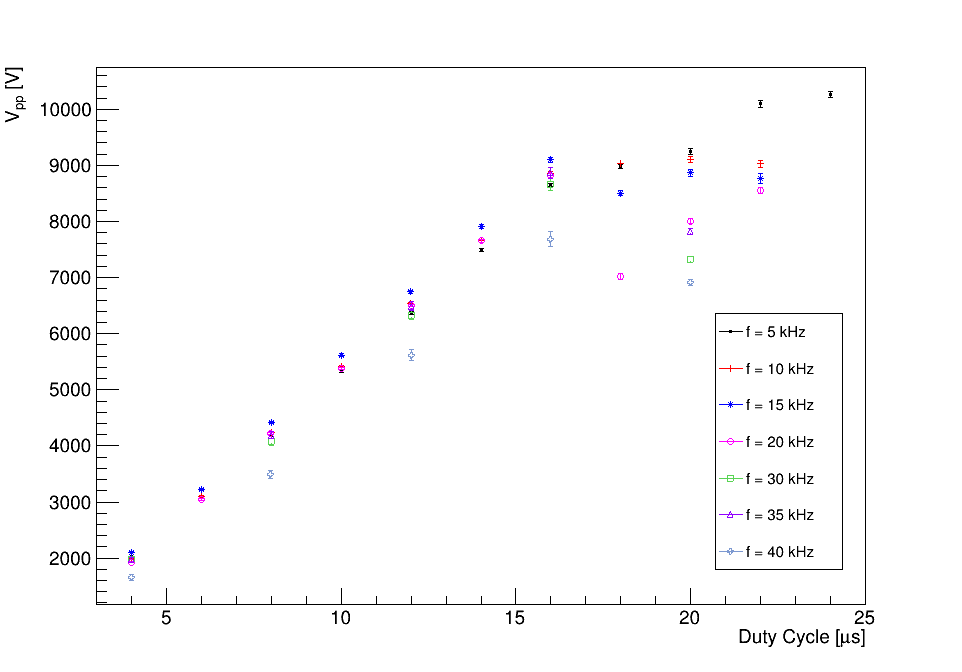
\includegraphics[width=.48\textwidth]{Immagini/nogas.png}}
\subfloat[][Misure con flusso di He $\SI{2}{\litre/\minute}$.]
  {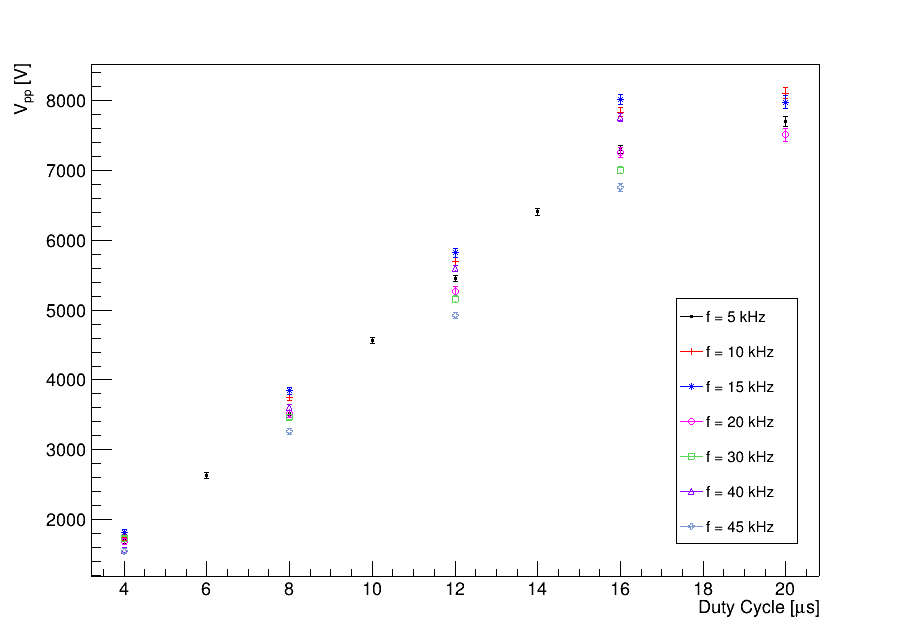
\includegraphics[width=.48\textwidth]{Immagini/gas.png}}
\caption{Tensioni di picco misurate al variare del tempo di apertura del circuito (Duty Cycle) e per diverse frequenze.}
\label{fig:tensioni}
\end{figure}


Vengono quindi calcolati i coefficenti dell'interpolazione lineare per le varie frequenze, presentati in figura \ref{fig:fitlin}. 
Come si può vedere i parametri non presentano un andamento specifico, sono disposti in modo casuale rispetto la loro media. Questo porta a concludere che non vi sia una dipendenza del funzionamento del circuito dalla frequenza.

Nell'analisi così proposta, viene ignorato che considerando l'errore associato alla stima dei parametri, i valori risultano incompatibili con un valore medio costante. Questo perché gli errori risultanti sono molto sottostimati: gli errori maggiori sono dovuti alle oscillazioni del picco principale al momento della misura, per migliorare la stima del picco bisognerebbe prendere più set di dati per ogni tempo di apertura del circuito.

\begin{figure}
\centering
\subfloat[][Pendenza delle rette.]
  {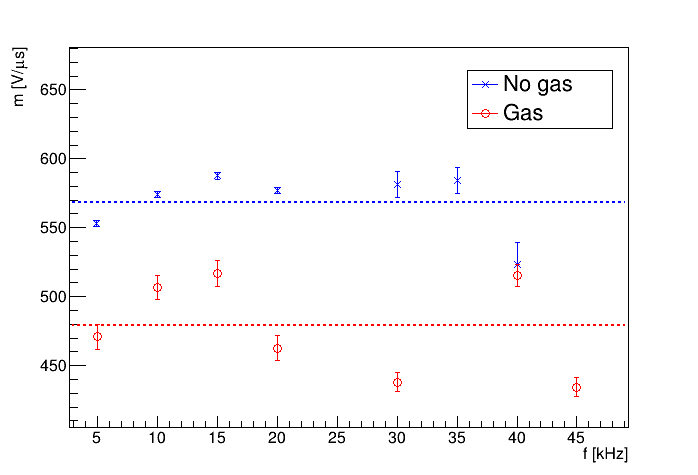
\includegraphics[width=.48\textwidth]{Immagini/m_freq_tot.png}}
\subfloat[][Intercetta delle rette.]
  {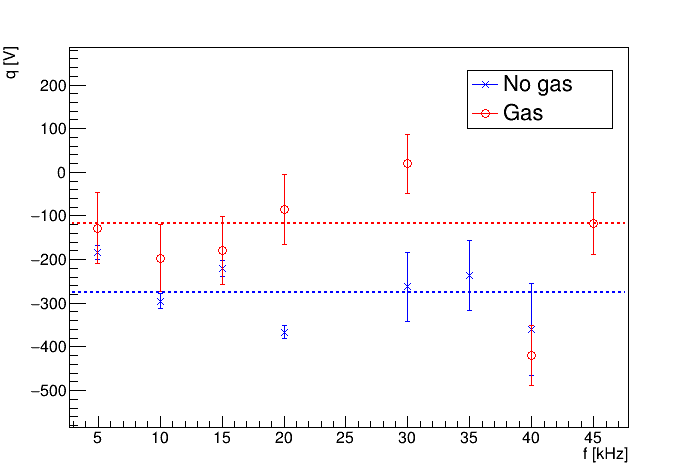
\includegraphics[width=.48\textwidth]{Immagini/q_freq_tot.png}}
\caption{Parametri dell'interpolazione lineare dei set di misure nel range, al variare della frequenza.}
\label{fig:fitlin}
\end{figure}

\paragraph{Corrente}L'analisi proposta è uguale a quella pensata per i set di misure precedenti: vengono tagliate le oscillazioni ad alta frequenza, ricostruito il segnale (aggiungendo l'errore dovuto al taglio delle alte frequenze e agli strumenti di misura) e il valore del minimo viene trovato interpolando con una funzione di Landau. Da questo fit vengono calcolati valori e posizione di picco di tensione, picco di corrente primario e picco di corrente secondario.
In figura \ref{fig:landau} un esempio del fit.

\begin{figure}
\centering
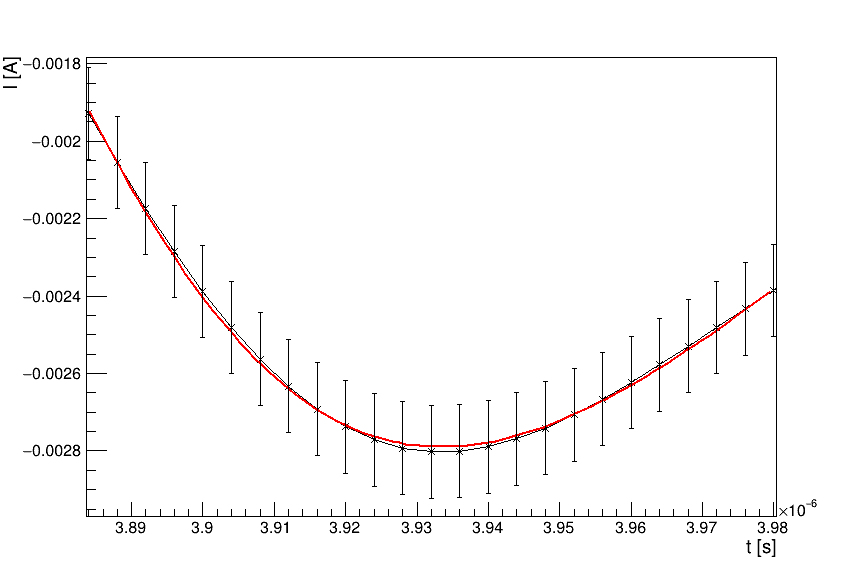
\includegraphics[width=.6\textwidth]{Immagini/es_fit_landau.png}
\caption{Esempio di fit del picco di corrente, $f = \SI{5}{\kilo\hertz}$ e $\Delta t = \SI{24}{\micro\second}$}
\label{fig:landau}
\end{figure}

Le tensioni del picco così calcolate, al variare della duty cycle per le diverse frequenze, sono presentate in figura \ref{fig:picchi}.
Nuovamente troviamo un andamento lineare per la tensione di picco tra i $\num{4}$ e i $\SI{16}{\micro\second}$. Anche il picco primario di corrente presenta questo andamento lineare, mentre per il picco secondario non è possibile identificare un comportamento simile, i valori si disperdono in modo apparentemente casuale.

\begin{figure}
\centering
\subfloat[][Modulo del picco di tensione.]
  {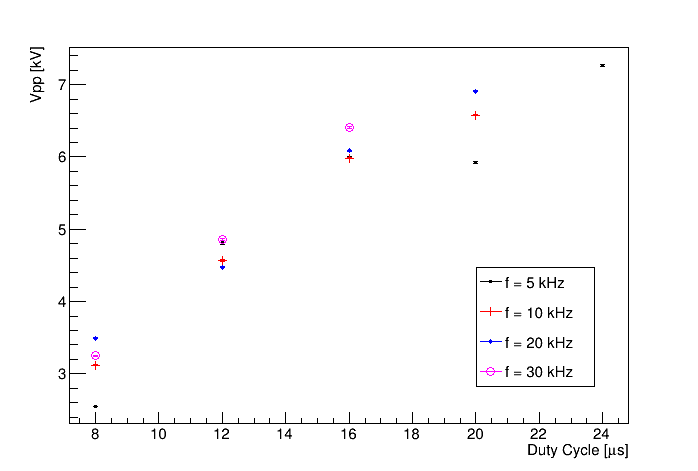
\includegraphics[width=.48\textwidth]{Immagini/vpp_corrente.png}}
\subfloat[][Modulo del picco primario di corrente.]
  {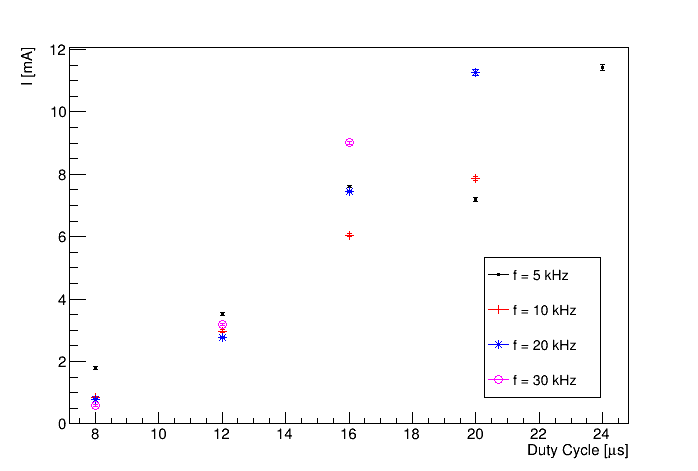
\includegraphics[width=.48\textwidth]{Immagini/I1_corrente.png}}
\newline
\subfloat[][Picco secondario di corrente.]
  {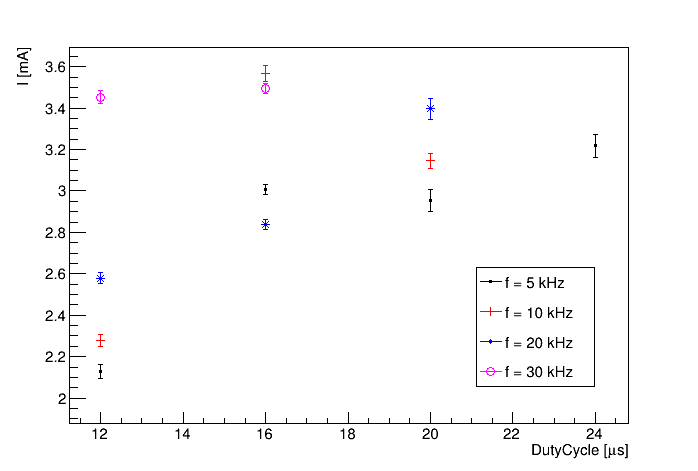
\includegraphics[width=.48\textwidth]{Immagini/I2_corrente.png}}
\caption{Valori dei picchi misurati al variare del tempo di apertura del circuito (Duty Cycle) e per diverse frequenze.}
\label{fig:picchi}
\end{figure}


Per il picco di tensione e il primo picco di corrente vengono quindi calcolati i coefficenti dell'interpolazione lineare delle diverse frequenze, presentati in figura \ref{fig:fitlin_cor}. 
Per i picchi di tensione nuovamente non viene trovato un andamento specifico dei parametri, i valori si assestano attorno una media lievemente inferiore rispetto le misure riportate precedentemente.
Per i picchi di corrente invece viene riscontrato un aumento della pendenza della retta all'aumentare della frequenza, sembrerebbe che a frequenze più elevate la corrente salga più velocemente aumentando il tempo di chiusura del circuito.

In ogni caso sono stati presi pochi set di misure, volendo concentrarsi sull'ordine di grandezza di tensione e corrente all'uscita dalla sorgente, un numero insufficiente per l'analisi di questi effetti.


\begin{figure}
\centering
\subfloat[][Pendenze dei picchi di tensione.]
  {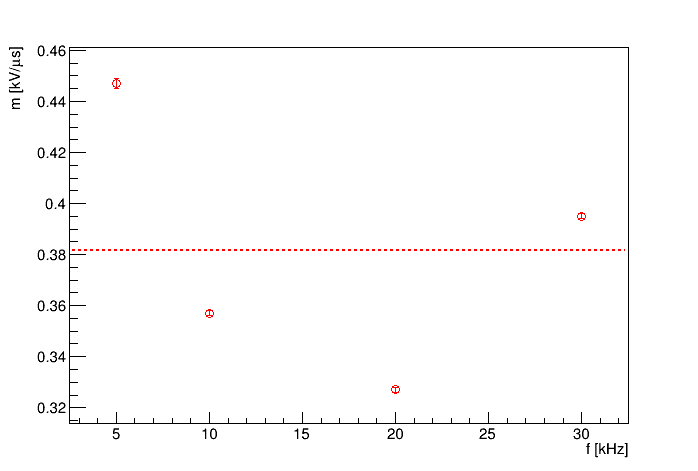
\includegraphics[width=.48\textwidth]{Immagini/mVpp_cor.png}}
\subfloat[][Intercette dei picchi di tensione.]
  {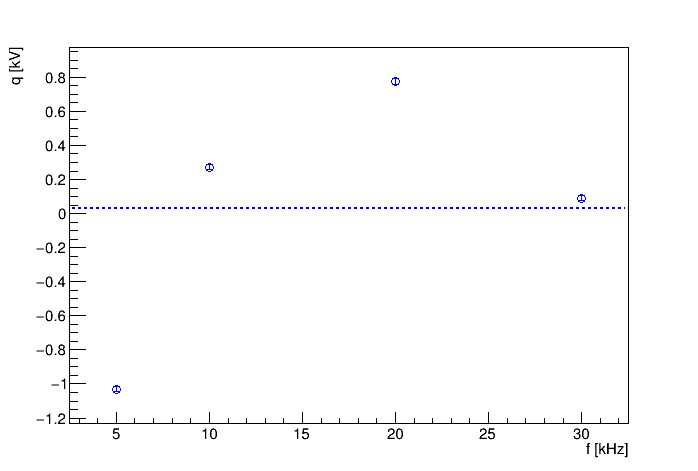
\includegraphics[width=.48\textwidth]{Immagini/qVpp_cor.png}}
\newline
\subfloat[][Pendenze dei picchi di corrente.]
  {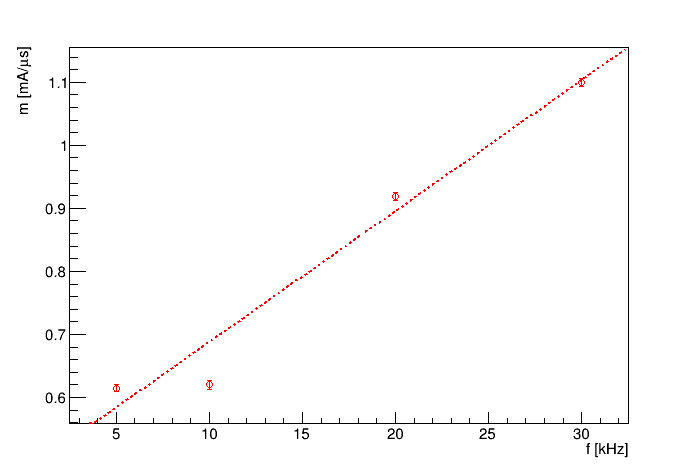
\includegraphics[width=.48\textwidth]{Immagini/mI1_cor.png}}
\subfloat[][Intercette dei picchi di corrente.]
  {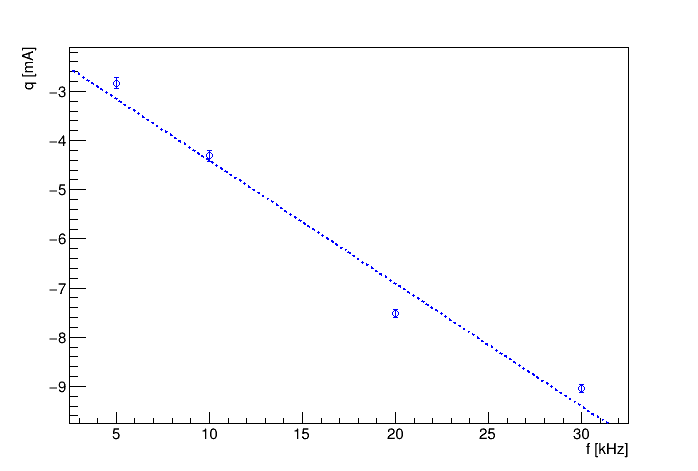
\includegraphics[width=.48\textwidth]{Immagini/qI1_cor.png}}
\caption{Parametri dell'interpolazione lineare dei picchi delle misure di tensione e corrente.}
\label{fig:fitlin_cor}
\end{figure}

Data la possibilità di visualizzare contemporaneamente sia la tensione sia la corrente in uscita dal circuito, viene proposta un'analisi delle variazioni temporali tra i diversi picchi. In particolare viene calcolato il tempo tra i due picchi di corrente e tra il picco di tensione e il picco di corrente primario, mostrati in figura \ref{fig:tempi}.
In entrambi i casi non è possibile estrapolare un andamento particolare, indicando che non vi sono differenze significative nei tempi di salita dei picchi al variare del tempo di apertura del circuito e della frequenza.

\begin{figure}
\centering
\subfloat[][Tempo tra i picchi di corrente.]
  {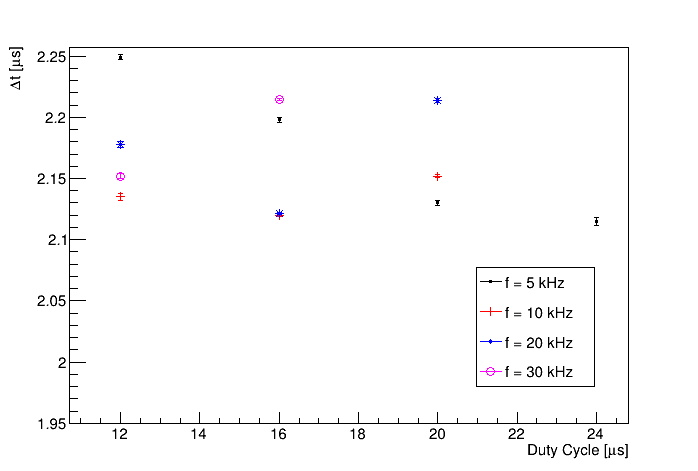
\includegraphics[width=.48\textwidth]{Immagini/ti2ti1.png}}
\subfloat[][Tempo tra picco tensione e primo picco di corrente.]
  {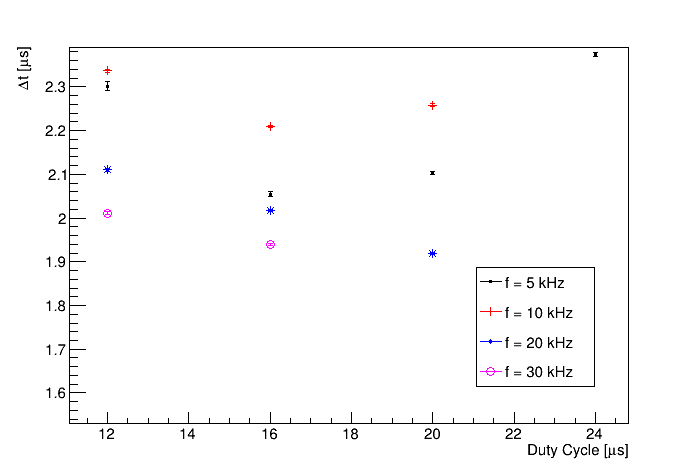
\includegraphics[width=.48\textwidth]{Immagini/ti1tv.png}}
\caption{Misura delle differenze temporali tra i picchi.}
\label{fig:tempi}
\end{figure}


\label{ch:discussione}
